\chapter{Alpha Wave: inhibition signal}
\label{chapter:four}
\epigraph{The electroencephalogram represents a continuous curve with continuous oscillations in which... one can distinguish larger first order waves with an average duration of 90 milliseconds...}{Berger}

This Chapter describes the experiments performed over a well-established but still mysterious EEG cognitive signal: The Berger Rhythm or Visual Occipital Alpha Waves.  An own dataset of resting subjects while maintaining their eyes open and closed is produced and the details of their generation are outlined.  Additionally, an experiment on a public Dataset will be also described.  Conclusions and discussion is described in the last section.

\section{Introduction}

%We gather the first dataset  using the EEG EPOC Emotiv Headset and we  access the raw signals using its C++ SDK provided by the manufacturer.  The device sends wirelessly  digitalized 128 Hz sampled EEG information as discrete packets.  Every packet is numbered and the electronic impedance is constantly measured, and delivered as part of the packet information. The wireless transmitter connects to a standard RF dongle which receives the information from  14 channels and forwards it into the PC, particularly to a custom C++ EEG Datalogger program that was developed in-house.  The program is waiting passively until a new packet is received from the dongle, verifying the packet numbering and controlling that the impedance is bellow a certain level, according to the device's documentation \cite{c11}. 

Alpha Waves were the first signals ever spotted from the Electroencephalography.  They are very well characterized as 10 Hz signals, physiologically consistent across subjects, and they are associated with synchronous inhibitory processes and attention shifting~\cite{c3}. They tend to be more prominent while subject's eyes are closed and appear stronger in occipital regions, around $O_1$ and $O_2$~\cite{c6,c11}. 

Figure BAL shows two records of 8 channels signals.  The signals in Figure BAL(a) contains the registered alpha waves with open eyes while the (b) contains the same information with their eyes closed.  The characteristic pattern of wiggles what was cough can be spotted, particularly for the Figure BAL(b).

This important rhythm is an oscillatory process.  As such, it is understood and studied in the frequency-domain.   Figure~\ref{fig:alphaspectrum} show the results of applying the Fast Fourier Transform to two different segments of $10\si{\seconds}$ length.  For each segment, the Power Spectral Density is calculated and their values are shown on the vertical axis.  Frequency values are shown on the horizontal axis.   On Figure (a) there isn't any particular frequency component.  However, on Figure (b) the prevalence of the 10 \si{\hertz} alpha wave component can be observed.   
 
It is also called the Posterior Dominant Rhythm due to their pervasiveness in EEG. 
 
%As can be seen in Fig. , if we process the Drowsiness dataset with a 8-12Hz band-pass filter and calculate the average power spectral density across subjects and for each channel, we can see how clearly the value corresponding to class 2 (eyes closed) is always higher than the value for class 1 (eyes open), confirming the expected result.  This also verifies how the differentiation information is contained mostly in the frequency-domain.

\begin{figure}[h!]
\centering
\subfigure[Subject was sit, relaxed in front of the Computer Monitor with his eyes open.]
{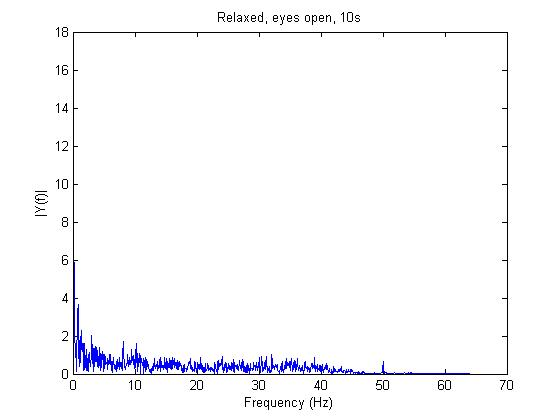
\includegraphics[height=5cm,width=7.5cm]{images/spectrumeyesopenO2.jpg}}
\subfigure[Subject was sit, relaxed in front of the Computer Monitor with his eyes closed. A strong $10 \si{Hz}$ component can be observed.]
{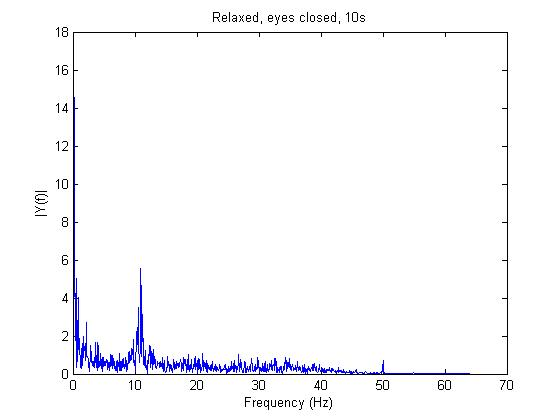
\includegraphics[height=5cm,width=7.5cm]{images/spectrumeyesclosedO2.jpg}}
\caption[Spectrum components obtained by the FFT of Alpha Waves]{Spectrum components of a $10 \si{s}$ signal segment of a subject with their eyes open. Data was obtained with OpenBCI device.}
\label{fig:alphaspectrum}
\end{figure}


%   \begin{figure}[thpb]
%      \centering
%      \setlength\fboxsep{0pt}
%	  \setlength\fboxrule{0.5pt}
%      \fbox{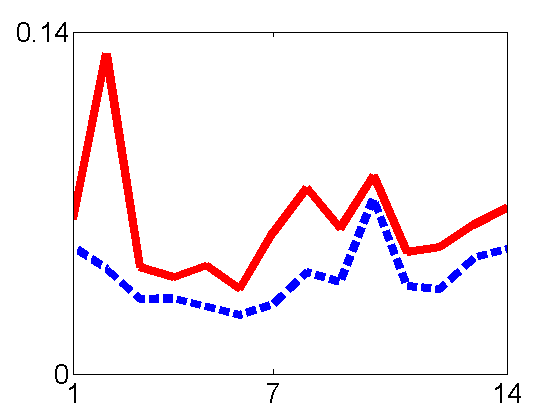
\includegraphics[width=2.5cm, height=1.8cm]{images/PSDExperiment1VsExperiment5.png}}
%      \fbox{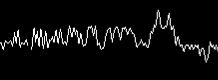
\includegraphics[width=2cm, height=1.8cm]{images/s_1_e_1_c_7_4.png}}
%      \caption[Power Spectral Density of Alpha Waves]{PSD values for every channel (x-axis) are being shown for class 1, dashed line, and class 2, solid line, for Dataset I (left). Sample EEG plot image corresponding to the subject 1 (center) for class 1 (eyes open), for the channel 7 ($ O_1 $) }
%      \label{figure1}
%   \end{figure}
   
\section{Materials and Methods}

\subsection{EPOC Emotiv alpha waves own dataset}
We gather the first dataset using the EEG EPOC Emotiv Headset using the C++ SDK library provided by the manufacturer and an in-house developed software program. The device has 14 channels, and a sampling rate of 128 Hz \cite{c11}. Ten healthy subjects between ages 20-50 were recruited and they accepted to wear the device and to participate in the experiments.  A 30 minutes procedure was required to adjust the headset to each user, in order to decrease the impedance on each electrode (bellow $5 \si{\kilo\ohm}$).  Once the set up was finished, each subject was instructed to sit in a relaxed position. Subsequently, she/he was instructed to watch the screen for 15 seconds, trying to avoid, as much as possible, to abruptly move its body or head.  During that time, a single-trial of 10 seconds-length window of EEG signals data was transferred to a PC and logged into standard binary files. After a 5 minutes pause, the subject was asked to close the eyes avoiding any movement while keeping the same pose for another batch of 15 seconds.  Again, 10 seconds of EEG information were transferred and logged into the PC. This finally gave us a sample of 10 subjects,  2 trial per subject, one for each class, composed of 14 channels, 10-seconds length or 1280 samples per window. 

For this dataset, 10 windows of 1s for each class were gathered from 10 healthy subjects.  Descriptors were extracted from all the generated images, from both classes, and they were used to classify images from the same set.       
      
\subsection{AlphaNet Dataset}
Additionally, we tested the method against the public dataset of the AlphaNet effort published by Schwartz group.


For the first two datasets, as the sampling frequency of both datasets is similar, Image and SIFT Descriptor Scale were adjusted to delta and gamma to 1.

What is remarkable, and will be is that the information is contained in the frequency domain.  How it was possible to obtain a fairly good accuracy with this method given that important point ?  The key here is the classification algorithm that was used across this thesis.  This is because the local information obtained from each descriptor "help" to balance a tendency of how the synchronous waves all behave, and that information get loaded into the class structure that is later exploited by the classification method.

\subsection{Dataset II - BCI Competition 2003 IV \textit{self-paced 1s}}
We validated our method against the "BCI Competition 2003, dataset IV \textit{self-paced 1s}" \cite{c51}. This dataset is composed of 28 channels, in 416 epochs of 50 samples per epoch (500 ms length at 100 Hz) each one with the corresponding label, where subjects were asked to type at will a letter on a keyboard with the right or left index finger.  It is based on the Bereitschaftspotential \cite{c52}, which is a Slow Cortical Potential, particularly a slow change in voltages towards a negative potential drift, around 1000-500 ms before the onset of the self-initiated movement.  In this case, the information lies strongly on the time-domain.

This dataset was recorded from a healthy subject during a no-feedback session. She/he sat in a normal chair with relaxed arms resting on the table and fingers in the standard typing position at the computer keyboard. The task was to press with the index and little fingers the corresponding keys in a self-chosen order and timing 'self-paced key typing'. The experiment consisted of 3 sessions of 6 minutes each. All sessions were conducted on the same day with some minutes break in-between. Typing was done at an average speed of 1 key per second.  

\section{Results}

As can be seen in Fig. \ref{psd}, if we process the Drowsiness dataset with a 8-12Hz band-pass filter and calculate the average power spectral density across subjects and for each channel, we can see how clearly the value corresponding to class 2 (eyes closed) is always higher than the value for class 1 (eyes open), confirming the expected result.  This also verifies how the differentiation information is contained mostly in the frequency-domain.

We process this Dataset with a 8-12 Hz band-pass filter, and calculate the Power Spectral Density across subjects for each channel.  In Fig. \ref{psd} it can be seen that the PSD value is greater for the class 2 (eyes closed), showing also that the differentiation information is contained mostly in the frequency-domain.

The results of applying a 8-12 Hz band-pass filter and calculating the Power Spectral Density (PSD) across subjects for each channel can be seen in Fig. \ref{figure1}, where the values obtained for class 2 (eyes closed) are higher than the values for class 1 (eyes open), showing that the differentiation information is contained in the frequency-domain.

   \begin{figure}[thpb]
      \centering
      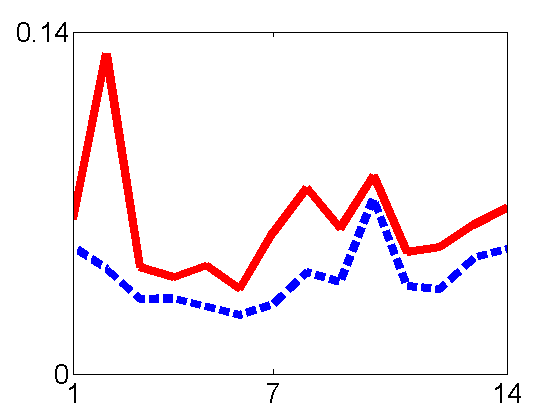
\includegraphics[scale=0.4]{images/PSDExperiment1VsExperiment5.png}
      \caption{Power Spectral Density band-passed at 8-12 Hz, for each channel.  The two experiments shows different levels and it can be seen how the experiment 2 for the Drowsiness Dataset has always higher values.  Channels are numbered according to the device numbering system which corresponds to specific electrodes of the 10-20 international system\cite{c6,c11}. }
      \label{psd}
   \end{figure}
   
   
\begin{figure}[h!]
\centering
\subfigure[A detailed image of a SIFT Descriptor over a plotted signal is shown.]
{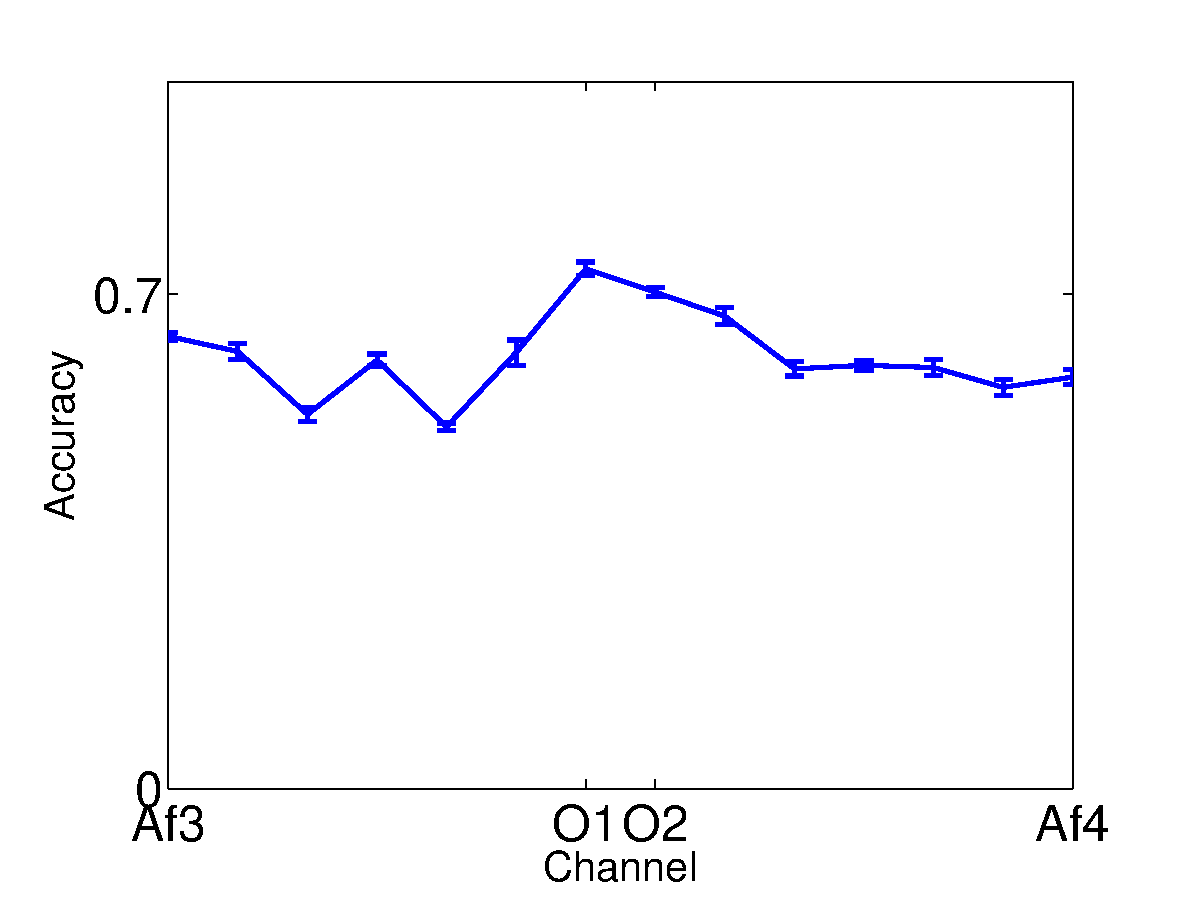
\includegraphics[width=7.5cm, height=5cm]{images/Dataset1AccuracyPerChannel}}
\subfigure[Classification Accuracy for discriminating windows of 1s (128 samples) of EEG signals from 10 subjects with their eyes open and closed.]
{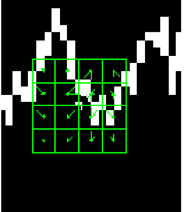
\includegraphics[width=7.5cm, height=5cm]{images/AlphaWaveSampleEEG.png}}
\caption[Alpha Waves Classification]{The classification accuracy is maximum on occipital channels O1 and O2. The descriptor size is 12x12 pixels which corresponds to a variation of 12 microvolts in the signal amplitude during 0.09 s.}
\label{fig:alpharesults}
\end{figure}
   
Regarding the first datasets, results were shown in Fig. 2 (right) where the classification accuracy is shown after applying a 10-Fold Cross Validation procedure on the entire set of labeled descriptors.  Descriptors from different subjects were used as part of the different training set to classify unknown images, so the obtained accuracy level was subject-independent.  Moreover, a classification level with average above $70\%$ was obtained in Occipital channels.


Spatial information based on accuracy

  \begin{figure}[thpb]
      \centering
      \setlength\fboxsep{0pt}
	  \setlength\fboxrule{0.5pt}
      \fbox{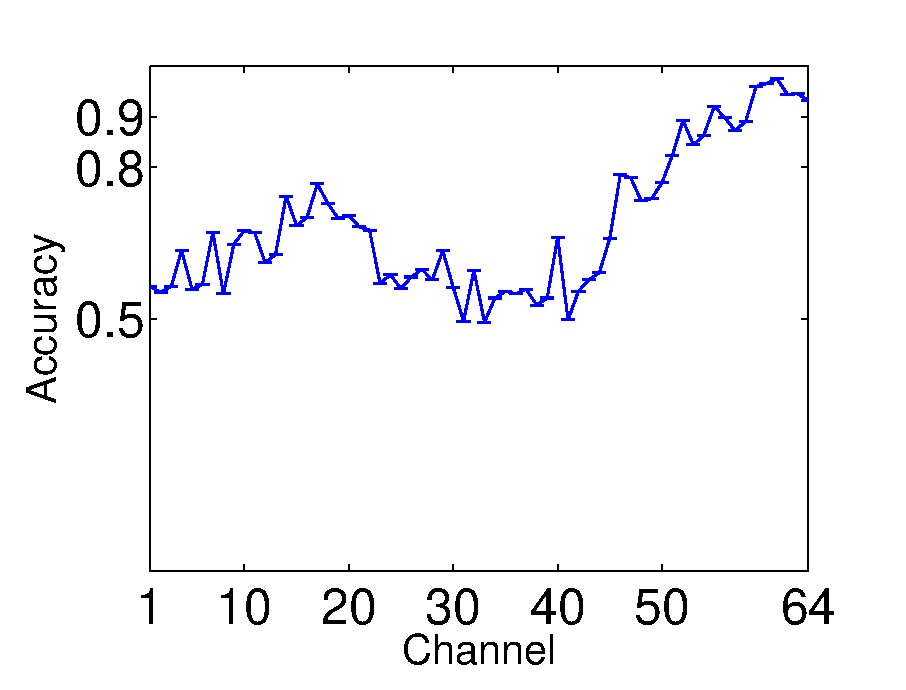
\includegraphics[width=7.5cm, height=5cm]{images/DatasetPhysionetAccuracyPerChannel}}
      \fbox{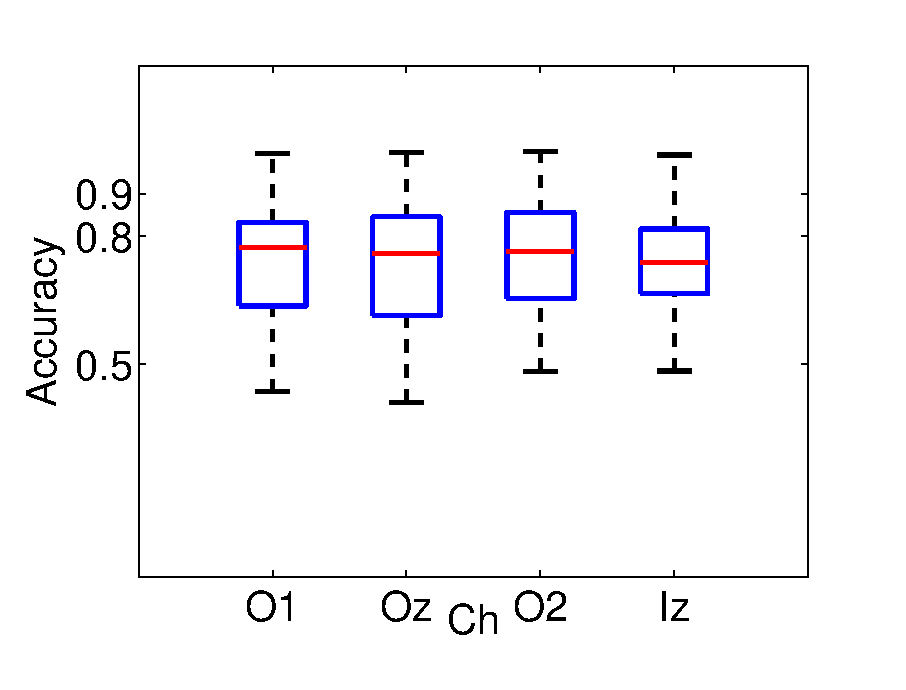
\includegraphics[width=7.5cm, height=5cm]{images/DatasetPhysionetBoxPlots}}
      \caption[Classification Accuracy of Alpha Waves]{Classification Accuracy for discriminating windows of 1s (160 samples) of EEG for Alpha Waves differences between subjects with eyes opened and closed. The descriptor size is 12x12 pixels. (Left) 10-Fold cross validated accuracies for one subject.  (Right) Average accuracy levels for 25 subjects for the occipital channels. Medians were above $75\%$.}
      \label{figure1}
   \end{figure}   

For the second dataset, an accuracy median higher than $70\%$ for 25 subjects, also on occipital channels O1, Oz, O2 and Iz (numbered 61 to 64) was obtained while discriminating Runs 1 and 2 (Baseline eyes open vs Baseline eyes closed). Fig. 3 shows the 10-Fold Validated Accuracy for one random subject [6,7], where a higher accuracy in the classification of the signals can also be seen with occipital channels.  

\section{Conclusion}

This results was surprassing.  We are using a method which is based on the waveform do detect a process which happens to be more prominent in spectrum.  But this shows at the same time the complex relationshipt between time and frequency.  The shape in time of a an oscilatory process prominent in frequency is clearly evident.  This goes in line with the fact that alpha waves can be seen in the EEG, and are basic tools of clinical diagnosis.

The posterior rythm is very important to assess healthy EEG patterns.


Although EPOC Emotiv is a commercial device, more apt as HCI tool, it is possible to detect fairly some BCI components.

Covert Spatial visual Attention